%	Autor:		Giuliano Montorio & Hannes Dittmann
%	Datum:		28.08.2018
%	Short:		Entwicklungsprojekt
% DOCUMENTCLASS -----------------------------------------------------------------------------------------
\documentclass[12pt,a4paper,oneside,numbers=noenddot,headsepline,captions=tableheading,toc=bibliography,openany,tikz,margin=5mm]{scrbook}
\usepackage{amsmath} 
\setcounter{secnumdepth}{5}
\renewcommand{\arraystretch}{1.4} 

% alles in helvetica
\renewcommand{\familydefault}{\sfdefault}



\usepackage{geometry}
\geometry{a4paper,left=25mm,right=25mm, top=25mm, bottom=25mm, includeheadfoot}
%\usepackage[scaled = 0.9]{helvet}

% SPRACHE------------------------------------------------------------------------------------------------
\usepackage[utf8]{inputenc}
\usepackage[autostyle,babel,german=guillemets,style=german]{csquotes}
\usepackage[USenglish,ngerman]{babel} 
\selectlanguage{ngerman}


% TABELLEN-----------------------------------------------------------------------------------------------
\usepackage{multirow} % Tabellen-Zellen �ber mehrere Zeilen1
\usepackage{multicol} % mehre Spalten auf eine Seite
\usepackage{makecell}
\usepackage{tabularx} % F�r Tabellen mit vorgegeben Gr��en
\usepackage{array}
\usepackage{float}
\usepackage{booktabs}
\usepackage{longtable} % Tabellen �ber mehrere Seiten
\usepackage{rotating}
\usepackage[table,xcdraw]{xcolor}
\usepackage{subcaption}
\usepackage{tikz}
\usetikzlibrary{circuits.ee.IEC}
\usetikzlibrary{positioning,calc,shapes,arrows,shapes.multipart}
\usepackage{pgfplots}
\pgfplotsset{
	dirac/.style={
		mark=triangle*,
		mark options={scale=2},
		ycomb,
		scatter,
		visualization depends on={y/abs(y)-1 \as \sign},
		scatter/@pre marker code/.code={\scope[rotate=90*\sign,yshift=-2pt]}
	}
}
\usetikzlibrary{arrows.meta,positioning,calc,scopes}
\def\iangle{0} % Angle of the inclined plane

\def\down{0}
\def\arcr{0.5cm} % Radius of the arc used to indicate angles
\usepackage{pdflscape}

% BILDER-------------------------------------------------------------------------------------------------
\usepackage{graphicx}
\usepackage{color}
\usepackage{svg}
\usetikzlibrary{arrows, shapes, 3d, calc, fit, positioning}
\usepackage{lipsum}
\usepackage{docmute}
\usepackage{graphicx}


% ALLGEMEINES--------------------------------------------------------------------------------------------
\usepackage{amsmath,amssymb} % Mathesachen
\usepackage[T1]{fontenc} % Ligaturen, richtige Umlaute im PDF
\usepackage[scaled = 0.9]{helvet}
\usepackage{url}		% bricht lange URLs ?sch�n? um [hyphens,obeyspaces,spaces]
\usepackage[decimalsymbol=comma]{siunitx}
\usepackage[onehalfspacing]{setspace}
\setlength{\parindent}{0cm}	% Disable automatic parindent
\usepackage{placeins}
\sloppy
\usepackage{mathrsfs}
\usepackage{xcolor}
\usepackage{pdfpages}
\usepackage{enumitem}
\graphicspath{{_img/}}
% PDF-----------------------------------------------------------------------------------------------------
\usepackage{pdfpages}
\usepackage[ngerman,%
pdfauthor={Giuliano Montorio},%
pdftitle={Masterarbeit G. Montorio},%
colorlinks=true,linkcolor=black,citecolor=black,filecolor=black,urlcolor=black%
]{hyperref}

% ABKÜRZUNGEN --------------------------------------------------------------------------------------------
\usepackage[nohyperlinks]{acronym}


% BIBLATEX -----------------------------------------------------------------------------------------------
\usepackage[backend=bibtex,%
style=IEEEtran,%
bibstyle=numeric,%
citestyle=numeric,%
sorting=none,%
]{biblatex}
\bibliography{_bib/biblio}

%CONSENS--------------------------------------------------------------------------
\usetikzlibrary{shapes.symbols}
\definecolor{CSblueColor}{rgb}{0.8,.92549,1}
\definecolor{CSyellowColor}{rgb}{1,1,0.6}
\tikzstyle{CONSENSc} = [double arrow,text=black!40,draw=black!40,thick,double arrow head extend=.0cm,align=center,font=\scriptsize,double arrow tip angle= 120,minimum width=10mm,minimum height=25mm]
\tikzstyle{CONSENS} = [double arrow,text=black,draw=black,thick,double arrow head extend=.0cm,align=center,font=\scriptsize,double arrow tip angle= 120,minimum width=10mm,minimum height=25mm]
\tikzstyle{CONSENSlegend} = [double arrow,text=black, draw=black,thick,double arrow head extend=.0cm,double arrow tip angle= 120,minimum width=8.8mm,minimum height=4.35mm]
\tikzstyle{CONSENSsysc} = [CONSENSc,fill=CSblueColor!40]
\tikzstyle{CONSENSenvc} = [CONSENSc,fill=CSyellowColor!40]
\tikzstyle{CONSENSsys} = [CONSENS,fill=CSblueColor]
\tikzstyle{CONSENSenv} = [CONSENS,fill=CSyellowColor]
\tikzstyle{CONSENSlegendenv}=[CONSENSlegend,fill=CSyellowColor]
\tikzstyle{CONSENSlegendsys} = [CONSENSlegend,fill=CSblueColor]
\tikzstyle{CSarrowc} = [-{triangle 45},text=black!40,draw=black!40]
\tikzstyle{CSarrow} = [-{triangle 45},text=black,draw=black]
% QUELLCODE -------------------------------------------------------------------
\usepackage{listings}
\definecolor{mygreen}{RGB}{28,172,0} 		% color values Red, Green, Blue
\definecolor{mylilas}{RGB}{170,55,241}
\lstset{language=Matlab,%
	basicstyle=\footnotesize\ttfamily,
	breaklines=true,%
	morekeywords={matlab2tikz},
	keywordstyle=\color{blue},%
	morekeywords=[2]{1}, keywordstyle=[2]{\color{black}},
	identifierstyle=\color{black},%
	stringstyle=\color{mylilas},
	commentstyle=\color{mygreen},%
	showstringspaces=false,%without this there will be a symbol in the places where there is a space
	numbers=left,%
	numberstyle={\tiny \color{black}},% size of the numbers
	numbersep=9pt, % this defines how far the numbers are from the text
	emph=[1]{for,end,break},emphstyle=[1]\color{red}, %some words to emphasise
	%emph=[2]{word1,word2}, emphstyle=[2]{style},    
}
\usepackage{nicematrix}
\usepackage{varwidth}
\newcommand\UmbruchConsens[2][2cm]{\begin{varwidth}{#1}\centering#2\end{varwidth}}
\newcommand\Umbruch[2][2cm]{\begin{varwidth}{#1}\centering#2\end{varwidth}}
\usepackage{makecell}

\usepackage{eqparbox}
\usetikzlibrary{matrix,positioning,arrows.meta,bending}
\newbox\matrixcellbox
\tikzset{math center align per column/.style={nodes={execute at begin
			node={\setbox\matrixcellbox=\hbox\bgroup$},
			execute at end
			node={$\egroup\eqmakebox[\tikzmatrixname\the\pgfmatrixcurrentcolumn][c]{\copy\matrixcellbox}}}},
	math center align per matrix/.style={nodes={execute at begin
			node={\setbox\matrixcellbox=\hbox\bgroup$},
			execute at end
			node={$\egroup\eqmakebox[\tikzmatrixname][c]{\copy\matrixcellbox}}}},
	3d matrix/.style={matrix of nodes,nodes in empty cells,math center align per
		matrix,nodes={draw,anchor=center,outer sep=0pt,inner sep=1pt,
			text height={height("\raisebox{0.2ex}{A}")},text depth={depth("g")}},
		column sep=-\pgflinewidth,row sep=-\pgflinewidth,execute at end matrix={
			\foreach \XX in {1,...,\the\pgfmatrixcurrentcolumn}
			{\draw (\tikzmatrixname-1-\XX.north east) -- ++ (#1,#1);}
			\ifnum\the\pgfmatrixcurrentrow>1
			\foreach \XX in {1,...,\the\numexpr\the\pgfmatrixcurrentrow-1}
			{\draw (\tikzmatrixname-\XX-\the\pgfmatrixcurrentcolumn.south east) -- ++ (#1,#1);}
			\fi
			\draw (\tikzmatrixname-1-1.north west) -- ++ (#1,#1) -- 
			([xshift=1ex,yshift=1ex]\tikzmatrixname-1-\the\pgfmatrixcurrentcolumn.north east) --
			([xshift=1ex,yshift=1ex]\tikzmatrixname-\the\pgfmatrixcurrentrow-\the\pgfmatrixcurrentcolumn.south east)  --
			(\tikzmatrixname-\the\pgfmatrixcurrentrow-\the\pgfmatrixcurrentcolumn.south east); 
	}},3d matrix/.default=1ex,
	Rightarrow/.style={double,double
		distance=#1,>={Implies[bend]},shorten <=0.4ex},Rightarrow/.default=1ex}




	
%Anfang PAP
\tikzset{
	papDecision/.style = {
		diamond,
		draw, 
		text width = 23 mm, 
		%align = flush left, 
		%text centered,
		inner sep = -2 pt,
		%font=\helvet,
		%line width = 1,
		minimum width = 30mm,
		minimum height = 7mm,
	},
	papStart/.style = {
		rectangle,
		draw, 
		align = center, 
		text width = 3cm, 
		text badly centered,
		inner sep = 4 pt,
		rounded corners=10pt,
		%font=\ttfamily\footnotesize,
		%line width = 1,
		minimum width = 30mm,
		minimum height = 7mm,
	},
	papEnd/.style = {
		rectangle,
		draw, 
		align = center, 
		text width = 3cm, 
		text badly centered,
		inner sep = 4 pt,
		rounded corners=10pt,
		%font=\ttfamily\footnotesize,
		%line width = 1,
		minimum width = 30mm,
		minimum height = 7mm,
	},
	papData/.style = {
		trapezium,
		draw, 
		align = center, 
		text width = 20 mm, 
		text badly centered,
		inner sep = 4 pt,
		trapezium left angle=70,
		trapezium right angle=110,
		%font=\ttfamily\footnotesize,
		%line width = 1,
		minimum width = 30mm,
		minimum height = 7mm,
	},
	papPredProc/.style = {
		draw,
		rectangle split,
		rectangle split horizontal,
		rectangle split parts = 3,
		rectangle split empty part width=-8pt,
		align = center, 
		%       text width = 4.5 em, 
		text badly centered,
		%        inner sep = 4 pt,
		%font=\ttfamily\footnotesize,
		%line width = 1,
		minimum width = 30mm,
		minimum height = 7mm,
	},
	papProcess/.style = {
		rectangle,
		draw,
		align = center, 
		text width = 3cm, 
		text badly centered,
		%inner sep = 2 pt,
		%font=\ttfamily\footnotesize,
		%line width = 1,
		minimum width = 30mm,
		minimum height = 7mm,
	},
	papLine/.style = {
		draw,
		-stealth,
		%font=\ttfamily\footnotesize,
		%line width = 1,
	},
}
\newcommand{\papYes}{ja}
\newcommand{\papNo}{nein}
%Ende PAP
	
\usepackage{tikz}
\usetikzlibrary{matrix,chains,positioning,decorations.pathreplacing,arrows}
% DOCUMENT ------------------------------------------------------------------------------------------------
\begin{document}
	
	%\pagestyle{empty}
	
	
	\cleardoublepage
	
	% ----------------------------------------------------------------------------------------------------------
	% TITELSEITE -----------------------------------------------------------------------------------------------
	% ----------------------------------------------------------------------------------------------------------
\begin{titlepage}
	\singlespacing
	
	
	\begin{figure}
		\centering
		\begin{minipage}[b]{0.5\textwidth}
			
\includegraphics[width=\textwidth]{Bilder/Logo_Smart_RGB}
			
		\end{minipage}
		\hfill
		\begin{minipage}[b]{0.4\textwidth}
			
\includegraphics[width=\textwidth]{Bilder/logo}
			
		\end{minipage}
	\end{figure}
	
	\begin{center}
		\vspace*{2cm}
		\Huge
		\textbf{Masterarbeit}\\
		\vspace*{0.5cm}
		\large
		zur Erlangung des akademischen Grades\\
		Master of Science (M.Sc.)\\
		\vspace*{2cm}
		\huge
		\textbf{Entwicklung einer Bildverarbeitung mit dem Schwerpunkt Personenerkennung für ein autonomes Logistik-Fahrzeug}\\
		\vspace*{1cm}
		\vfill
		\normalsize
		\newcolumntype{x}[1]{>{\raggedleft\arraybackslash\hspace{0pt}}p{#1}}
		
		\begin{tabular}{x{6cm}p{7.5cm}}
			\rule{0mm}{5ex}
			\textbf{Autor:} & Giuliano Montorio
			\newline giuliano.montorio@hs-bochum.de
			\newline Matrikelnummer: 015202887
			\newline\\
			
			
			\rule{0mm}{5ex}\textbf{Erstgutachter:} & Prof.\ Dr.-Ing.\ Arno Bergmann\\
			\rule{0mm}{2ex}\textbf{Zweitgutachter:} & M.Sc.\ Bernd Möllenbeck \\
			\rule{0mm}{5ex}\textbf{Abgabedatum:} & tt.mm.jjjj\\ 
		\end{tabular} 
	\end{center}
\end{titlepage}

	\onehalfspacing
	\cleardoublepage
	\cleardoublepage
	
	
	
	\chapter*{\textbf{Eidesstattliche Erklärung}}
	%\LARGE
	\textbf{Eidesstattliche Erklärung zur Abschlussarbeit:}
	\newline
	\newline
	\newline
	\flqq Entwicklung einer Bildverarbeitung mit dem Schwerpunkt Personenerkennung für ein autonomes Logistik-Fahrzeug\frqq
	\newline
	\newline
	\newline
	%\large
	Ich versichere, die von mir vorgelegte Arbeit selbstständig verfasst zu haben. Alle
	Stellen, die wörtlich oder sinngemäß aus veröffentlichten oder nicht veröffentlichten
	Arbeiten anderer entnommen sind, habe ich als entnommen kenntlich gemacht.
	Sämtliche Quellen und Hilfsmittel, die ich für die Arbeit benutzt habe, sind angegeben.
	Die Arbeit hat mit gleichem Inhalt bzw. in wesentlichen Teilen noch keiner anderen
	Prüfungsbehörde vorgelegen.
	\newline
	\newline
	\newline
	\newline
	\newline
	\newline
	\newline
	\newline
	\begin{center}
		\begin{tabular}[h]{lp{2cm}p{5.5cm}}
			Bochum, \today & & \\
			\cline{1-1}\cline{3-3}
			Ort, Datum& & Giuliano Montorio\\
		\end{tabular}
	\end{center}
	
	
	\chapter*{\textbf{Danksagung}}
	
	
	%\large
	
	Ein großes Dankeschön gilt all jenen Personen, die mich im Rahmen dieser Masterarbeit
	unterstützt und motiviert haben. Insbesondere möchte ich Herrn Prof. Dr.-Ing. Arno Bergmann, Herrn M.Sc. Bernd Möllenbeck und Herrn Dr.-Ing. Christoph Krimpmann danken, die meine Arbeit durch ihre fachliche und persönliche Unterstützung begleitet haben. Ich danke Guido Stollt und der gesamten Smart Mechatronics GmbH für die tolle Zusammenarbeit. Auch beim Fachbereich Elektrotechnik und Informatik der Hochschule Bochum, insbesondere Herrn Dipl.-Ing. Thorsten Bartsch möchte ich mich bedanken. Meiner Familie spreche ich meinen Dank aus, da sie mir mein Studium durch finanzielle, doch vor allem mentale Unterstützung ermöglicht haben. Bei meinem Bruder bedanke ich mich für die Bereitstellung seiner Räumlichkeiten für eine fortlaufende Entwicklung am autonomen Logistikfahrzeug während der Coronapandemie. Ein spezieller Dank gebührt Hannes Dittmann. Mit ihm habe ich nicht nur einen wegweisenden Mitstreiter gefunden, sondern auch einen tollen Freund.
	
	
	% ----------------------------------------------------------------------------------------------------------
	% VERZEICHNISSE --------------------------------------------------------------------------------------------
	% ----------------------------------------------------------------------------------------------------------
	\pagenumbering{roman}
	\tableofcontents
	\cleardoublepage
	
	
	
	\chapter*{Abkürzungsverzeichnis}
	\addcontentsline{toc}{chapter}{Abkürzungsverzeichnis}
	\begin{acronym}[CONSENS]% längste Abkürzung
		\acro{ALF}{\textbf{A}utonomes \textbf{L}ogistik \textbf{F}ahrzeug}		%\acro{Kuerzel}{Langform}
		\acro{CNN}{\textbf{C}onvolutional \textbf{N}eural \textbf{N}etworks}
		\acro{COCO}{\textbf{C}ommon \textbf{O}bjects in \textbf{Co}ntext}
		\acro{CONSENS}{\textbf{Con}ceptual Design \textbf{S}pecification Technique for the \textbf{En}gineering of Complex \textbf{S}ystems}
		\acro{cuDNN}{\textbf{CU}DA \textbf{D}eep \textbf{N}eural \textbf{N}etwork}
		\acro{EA}{\textbf{E}ndlicher \textbf{A}utomat}
		\acro{FN}{\textbf{F}alse \textbf{N}egative}
		\acro{FP}{\textbf{F}alse \textbf{P}ositive}
		\acro{FPS}{\textbf{F}rames \textbf{P}er \textbf{S}econd}
		\acro{HOG}{\textbf{H}istogram of \textbf{O}riented \textbf{G}radients}
		\acro{IoU}{\textbf{I}ntersection \textbf{o}ver \textbf{U}nion}
		\acro{KI}{\textbf{K}ünstliche \textbf{I}ntelligenz}
		\acro{KNN}{\textbf{K}ünstliches \textbf{N}euronales \textbf{N}etz}
		\acro{LiDAR}{\textbf{Li}ght \textbf{D}etection \textbf{A}nd \textbf{R}anging}
		\acro{mAP}{\textbf{M}ean \textbf{A}verage \textbf{P}recision}
		\acro{MMI}{\textbf{M}ensch-\textbf{M}aschine-\textbf{I}nterface}
		\acro{ReLU}{\textbf{Re}ctifier \textbf{L}inear \textbf{U}nit}
		\acro{ROS}{\textbf{R}obot \textbf{O}perating \textbf{S}ystem}
		\acro{SAE}{\textbf{S}ociety of \textbf{A}utomotive \textbf{E}ngineers}
		\acro{SSD}{\textbf{S}ingle \textbf{S}hot Multibox \textbf{D}etector}
		\acro{SVM}{\textbf{S}upport \textbf{V}ector \textbf{M}achine}
		\acro{TN}{\textbf{T}rue \textbf{N}egative}
		\acro{TP}{\textbf{T}rue \textbf{P}ositive}
		\acro{SLAM}{\textbf{S}imultaneous \textbf{L}ocalization \textbf{A}nd \textbf{M}apping}

			
	\end{acronym}
	\cleardoublepage
	%
	\pagestyle{plain}
	
	\chapter*{Symbolverzeichnis}
	\addcontentsline{toc}{chapter}{Symbolverzeichnis}
	
	\begin{longtable}{p{3cm}p{8cm}}
		\setlength\tabcolsep{9pt}
		Symbol & Bedeutung \\ \hline
		\endfirsthead
		Symbol & Bedeutung \\ \hline
		
		\endhead
		\toprule 
		$D_\text{F}$&Dimension der Eingangsdaten\\
		$D_\text{K}$&Dimension des Kernels\\
		$F$&veränderte Bilddaten\\
		$FN$&Anzahl aller False Positive Werte\\
		$FP$&Anzahl aller False Negative Werte\\
		$H$&Neuron einer versteckten Schicht\\
		$I$&Neuron einer Eingabeschicht\\
		$K$&Anzahl aller Klassen\\
		$N$&Tiefe der Ausgangsdaten\\
		$M$&Tiefe der Eingansdaten\\
		$O$&Neuron einer Ausgabeschicht\\
		$R_\text{d}$&Rechenaufwand bei konventioneller Faltung\\
		$R_\text{m}$&Rechenaufwand bei tiefenorientierter, trennbarer Konvolution mit Weiten- und Auflösungsmultiplikatoren\\ 
		$R_\text{p}$&Rechenaufwand bei tiefenorientierter Faltung\\
		$R_\text{r}$&Reduktionsfaktor des Rechenaufwands\\
		$R_\text{t}$&Rechenaufwand bei tiefenorientierter, trennbarer Konvolution\\
		$TN$&Anzahl aller True Negative Werte\\
		$TP$&Anzahl aller True Positive Werte\\
		
		$b$&Bildbreite\\
		$d$&Distanz\\
		$d'$&Begrenzung der Distanz durch die Objektivebene\\
		$g$&Binärfunktion\\
		$i, j$&Neuron\\
		$k$&Knotenemenge\\
		$m$&Modusfunktion\\
		$p$&Precision\\
		$p_x$&laterale Positionskoordinate\\
		$p_x'$&Pixelkoordinate\\
		$p_y$&longitudinale Positionskooridinate\\
		$p_y'$&Begrenzung der longitudinalen Positionskoordinate durch die Objektivebene\\
		$r$&Recall\\
		$t$&Zeitschritt\\
		$x$&Bilddaten\\
		$w$&Gewichte	\\ 
		
		$\alpha$&Weitenmultiplikator\\
		$\beta$&Sichtwinkel\\
		$\gamma$&Ausgabe eines Zustandsautomats\\
		$\epsilon$&Zustand\\
		$\zeta$&Eingabe in Zustandsautomat\\
		$\rho$&Auflösungsmultiplikator\\	
		$\phi$&Transitionsfunktion\\
		$\psi$&Ausgabefunktion\\ \hline
		
		
		%-----------------------------Tabelle--------------------
		\bottomrule
	\end{longtable}
	
	
	
	\cleardoublepage
	\pagestyle{headings}
	\pagenumbering{arabic}
	\setlength{\parskip}{0.1em}
	% ----------------------------------------------------------------------------------------------------------
	% INHALT steht in "Inhaltsverzeichnis" ---------------------------------------------------------------------------------------------------
	% ----------------------------------------------------------------------------------------------------------
	
\chapter{Einleitung}
\label{ch: Einleitung}
	

		Das Thema der künstlichen Intelligenz (KI) dringt zunehmend in den Alltag des Menschen ein. Smart Home Geräte wie \textit{Amazons Alexa}, \textit{Siri} der Firma \textit{Apple} oder der \textit{Google Assistant} gehören mittlerweile in einer Vielzahl deutscher Haushalte \cite{bvdw}. Derartige Technologien begleiten den Menschen jedoch nicht nur Zuhause, sondern auch in der Transport- und Logistikbranche. Eine Potenzialanalyse zur künstlichen Intelligenz der Firma \textit{Sopra Steria} zeigt, dass bereits im Jahr 2017 20\% aller befragten Unternehmen derartige Systeme einsetzten \cite{sopra}. 37\% planten den zukünftigen Einsatz \cite{sopra}. Die Implementierung solcher Systeme hat Einfluss auf verschiedenste Eigenschaften der Wertschöpfungskette \cite{sopra}. Auch die Qualität der Fachprozesse...(fachprozesse) wird mit steigender Geschwindigkeit erhöht \cite{sopra}. Einige der zur Logistikbranche gehörenden Transportfahrzeuge sind ebenfalls mit KI...(KI inflationär) ausgestattet. Sie sorgen so für weniger Arbeitsunfälle und eine schnellere, präzisiere Abarbeitung der Logistikaufgaben.\\
		
		\begin{figure}[H]
			\begin{minipage}[b]{0.49\textwidth}
				(a)
				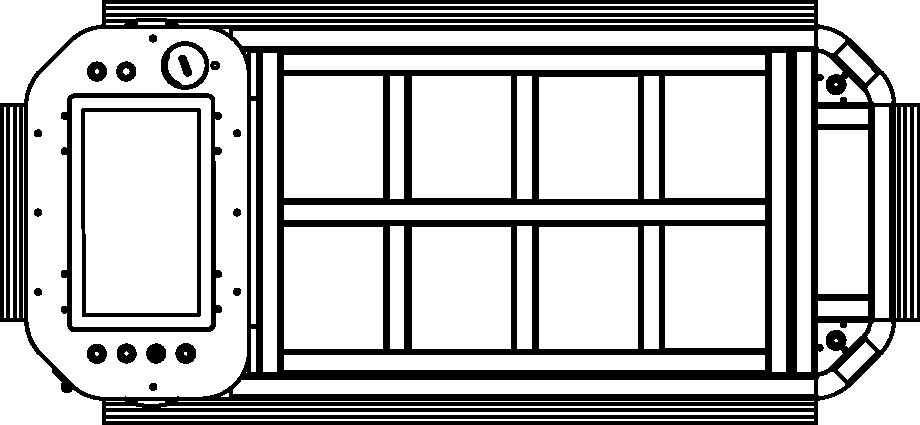
\includegraphics[width=0.9\textwidth]{Bilder/oben.pdf}
			\end{minipage}
			\begin{minipage}[b]{0.49\textwidth}
				(b)
				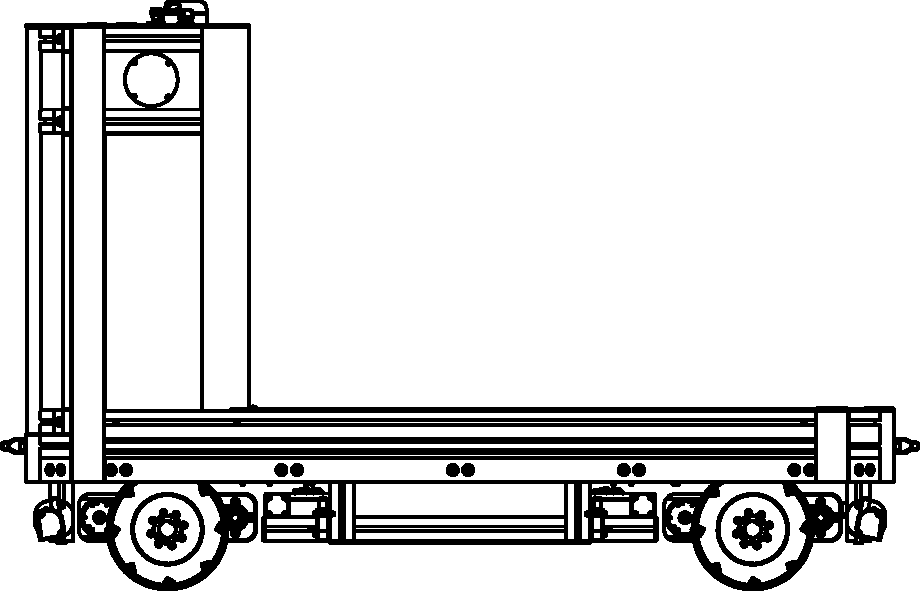
\includegraphics[width=0.9\textwidth]{Bilder/seite.pdf}
			\end{minipage}
			\centering
			\caption{(a) Darstellung des autonomen Logistik-Fahrzeugs aus der Draufsicht. Die acht benachbarten Rechtecke in der Mitte des Fahrzeugs stellen die Ladefläche des Fahrzeugs dar. (b) Darstellung aus der Seitenansicht. Oben links in der Abbildung ist der Schaltschrank zu sehen. Die Räder des Fahrzeugs befinden sich unten links und unten rechts in der Darstellung.}
			\label{fig: Darstellung des ALFs}
		\end{figure}
		
		Das autonome Logistikfahrzeug ALF ist ein solches Transportfahrzeug. Die Idee des ALFs ist es ein Fahrzeug zu entwickeln, das nach seiner Fertigstellung Logistikaufgaben am Standort der Hochschule Bochum lösen soll. Es dient im Labor für Antriebstechnik der Hochschule Bochum als Versuchs- und Entwicklungsplattform für praktische Anwendungen. Der Entwicklungsprozess stellt sich aus diversen Bachelor- und Masterarbeiten zusammen, die sowohl Hardware, als auch Softwareintegrationen vorsehen. Bisher wurden zwei Abschlussarbeiten inklusive der praktischen Anwendung am ALF geschrieben. M.Sc. Dennis Hotze und M.Sc. Dominik Eickmann entwickelten in ihrem Masterprojekt das Fahrzeug und konnten Fahraufgaben ferngesteuert und manuell erledigen. Während der darauffolgenden Bachelorarbeit wurde eine Schlupfkompensation entwickelt, die den Drift am Fahrzeug durch Eingabe von Umgebungsinformationen verhindert. Weiterhin wurden Funktionen entwickelt, um grundlegende und autonome Fahraufgaben zu lösen. Das autonome Logistikfahrzeug aus der vorangegangenen Bachelorarbeit dient auch in dieser Masterarbeit als Versuchsplattform.\\
		
		Der tägliche Kontakt zu Menschen ist nicht nur für den ALF, sondern auch für andere Transportfahrzeuge im öffentlichen Raum unentbehrlich. Kreuzen sich die Wege eines autonomen Fahrzeugs mit der einer oder mehrerer Personen, darf es in keinster Weise zur Kollision kommen. Je nach Dimension des Fahrzeugs können die Folgen fatal sein. Das ALF zählt mit einem Maximalgewicht von 600 kg zu der Art von Fahrzeugen, die bei einem Zusammenstoß besonders schwere Verletzungen hervorrufen kann. Ein solches System muss folglich in der Lage sein, bei Annäherung von Personen eine gesonderte Gefahreneinschätzung vorzunehmen. Im Einsatz an der Hochschule Bochum kommt es eher selten zu Begegnungen mit Tieren ohne der Begleitung von Personen. Dementsprechend wird das System im Rahmen dieses Projekts auf die Erkennung von Personen beschränkt. Ein weiteres, übliches Szenario solcher Systeme im öffentlichen Raum ist die Bedienung durch nicht autorisierte Personen. Für derartige Zwecke muss ein Mensch nicht nur als bewegtes Objekt, sondern auch als solcher erkannt werden. \\
		
		Am ALF sind zwei \textit{Kinect}-Kameras angebracht \cite{Bachelorarbeit}. Bisher wurde der Großteil der Funktionen dieser Kameras nicht verwendet. ...In der vorangegangenen Bachelorarbeit wurden dreidimensionale in zweidimensionale Tiefeninformationen umgewandelt, um ein Problem bedingt durch die Einbauhöhe der Kameras zu lösen \cite{Bachelorarbeit}. Das Hauptziel dieser Masterarbeit ist die Entwicklung einer Personenerkennung. Die genannten Kameras dienen neben eines \textit{Light Detection and Ranging} (LiDAR) Sensors als einzige optische Sensoren des autonomen Logistikfahrzeugs. Zwar gibt es technische Lösungen für eine Personenerkennung mithilfe von zweidimensionalen Laserdaten. Jedoch werden Menschen mithilfe von Bildverarbeitung deutlich genauer detektiert. Folglich wird das System zur Personenerkennung mithilfe der beiden \textit{Kinect} Kameras ausgelegt. Weiterhin soll das System nicht nur Personen detektieren können, sondern diese auch wiedererkennen. \\
		
		Während der Bearbeitung von Transport- oder Fahraufgaben eines autonomen Fahrzeugs kann es zu diversen Komplikationen kommen. Beispielsweise können besonders im Anwendungsbereich der Hochschule Bochum diverse Objekte den Verlauf einer Route unterbrechen und ein Ziel sogar unerreichbar machen. Häufig können diese Probleme durch menschliche Hilfe beseitigt werden. Wiederum setzt dies eine Interaktion mit umstehenden Personen vorraus. Eine Besonderheit dieser Masterarbeit ist die theoretische und praktische Entwicklung parallel zu einem weiteren Projekt. Hannes Dittmann entwickelt in seiner Masterarbeit eine Sprachverarbeitung zur Klassifikation anwendungsorientierter Sprache \cite{Dittmann}. Diese stellt eine auditive \textit{Mensch-Maschine-Interface} (MMI) Schnittstelle her. So kann eine Person über ein Aufnahmegerät mit dem System kommunizieren. Die klassifizierte Sprache ist ohne Weiteres nicht in der Lage das Fahrzeug enstprechend zu steuern.\\
		
		Demnach wird in dieser Masterarbeit ein Konzept zur Steuerung des ALFs mit klassifizierter Sprache entwickelt und am Fahrzeug implementiert. Darüber hinaus gilt es die Steuerung des Systems nach gegebenen Standards auszulegen. Die \textit{Society of Automotive Engineers} (SAE) ist eine Organisation, die aus über 128000 Ingenieuren und technischen Experten besteht \cite{saeorg}. Ziel dieser ist im Allgemeinen die Weiterentwicklung im Thema Mobilität \cite{saeorg}. Unter anderem veröffentlicht \textit{SAE International} Normen, wie die \textit{SAE J3016}. Diese beschäftigt sich mit verschiednen Stufen der Automatisierung von Fahrzeugen. Eine entsprechende Tabelle ist in Abbildung \ref{fig: tabautonom} dargestellt.\\
		
		Das ALF wird zum Zeitpunkt des Entwicklungsbeginns dieser Masterarbeit auf dem \textit{SAE-Level} 3 eingeschätzt. Hierbei werden lediglich die autonomen Fahrmodi des Fahrzeugs berücksichtigt. Die Fahrbefehle konnten selbstständig durch das System ausgeführt werden und die Umgebung über die bereits genannten, zweidimensionalen Laserdaten erfasst werden. Die \textit{Fallback Performance} beschreibt den Übergang des automatisierten oder autonomen in einen risikominimalen Zustand. Bisher musste die laufende Software des ALFs auch im Fehlerfall manuell am Fahrzeug beendet werden. Dies bestärkte die Einschätzung, dass das Fahrzeug bedingt automatisiert sei.	
		
		\newcolumntype{C}[1]{>{\centering\arraybackslash}p{#1}}
\newcolumntype{M}[1]{>{\centering\arraybackslash}m{#1}}
\begin{table}[H]
	\caption{Übersicht der sechs Automatisierungsstufen nach SAE Standard J3016. Die Angaben wurde von der Quelle übernommen und sind sinngemäß übersetzt. \cite{sae}  }
	\begin{center}
		\begin{tabular}{|M{10mm}|M{48mm}|M{20mm}|M{20mm}|M{15mm}|M{20mm}|}
			\hline
			SAE Level  & Name & Ausführung von Fahrbefehlen & Erfassung der Umgebung& Fallback Performance& System-auswirkung\\ \hline
			\multicolumn{6}{|c|}{Benutzer überwacht die Fahrumgebung}\\ \hline
			
			0	& Keine Automatisierung			&Benutzer   &Benutzer &Benutzer & k.A.	 \\ \hline
			1	& Assistiert					& Benutzer \& System &Benutzer &Benutzer & Einige Fahrmodi	 \\ \hline
			2	& Teilautomatisiert				& System 	 &Benutzer&Benutzer&Einige Fahrmodi	 \\ \hline
			\multicolumn{6}{|c|}{Automatisiertes System - System überwacht Fahrumgebung}\\ \hline
			3	& Bedingte Automatisierung		& System &System&Benutzer&Einige Fahrmodi	 \\ \hline
			4	& Hochautomatisiert			& System &System&System&Einige Fahrmodi	 \\ \hline
			5	& Vollautomatisiert (autonom)	& System&System&System&Alle Fahrmodi	 \\
		
			
			\hline
		\end{tabular}
	\end{center}

	\label{fig: tabautonom}
\end{table}
		
		Als weiteres Ziel dieser Masterarbeit wird das ALF im Rahmen der technischen und sicherheitsrelevanten Möglichkeiten auf das \textit{SAE-Level} 5 angehoben. Dies betrifft insbesondere die zu entwickelnde Steuerung des Fahrzeugs.\\
		
		Diese und die Masterarbeit von Hannes Dittmann bilden im praktischen Kontext ein überarbeitetes Gesamtsystem des bereits bestehenden autonomen Logistikfahrzeugs. Die genannten Ziele sind im angehängten Lastenheft festgehalten und haben somit einen anwendungsorientierten Hintergrund. Der Anspruch an das zu entwickelnde System, ist die Zielerreichung mittels wissenschaftlicher Methoden zu erarbeiten.  
		
		
	
	\chapter{Grundlagen}
\label{ch: Grundlagen}
	Für ein besseres Verständnis, der in Kapitel Konzept... angewandten Methoden, werden anbei die Grundlagen behandelt. Informationen zu der verwendeten Hard- und Software wurden bereits in der vorangegangenen Bachelorarbeit vermittelt. Aufgrund Anforderung A... ist während der praktischen Anwendung keine Änderung der Hardware vorgesehen.
 
	
 	\section{Neuronale Netze}
	\label{sec: ROS}
	
	Das Neuronennetz des menschlichen Gehirns dient als Vorbild für künstliche, neuronale Netze (KNN). Diese werden heutzutage als Lösung diverser Anwendungsprobleme angewendet, in denen komplexe Strukturen und Muster aus großen Datenmengen erkannt werden sollen. Das in diesem Projekt zugrundeliegende Bildverarbeitungsproblem besitzt die beschriebenen Eigenschaften und eignet sich somit für den Einsatz zur Erkennung von Personen. Anders als bei den meisten programmierten Applikationen ist die Ausgabe von KNN's lediglich probabilistisch. Beim vorliegenden, autonomen Logistikfahrzeug werden zur Personenerkennung derartige neuronale Netze verwendet.
	
		\subsection{Eigenschaften von neuronalen Netzen}
		
		Das Grundlage für die Eingabe in ein neuronales Netz ist die Skalierung der vorliegenden Daten auf eine definierte Größe. Diese wäre beispielsweise bei einem Anwendungsfall mit einer Audiospur die Frequenzspektren oder bei einem Bildverarbeitungsproblem die Pixel eines Bildes. Die skalierten Daten werden in einem Tensor gegeben der die Dimensionen der Eingabe hat. Somit unterteilt sich ein Bild in die drei Dimensionen, die Höhe, die Weite und die Farbwerte der Primärfarben pro Pixel.  
		
		/Bild Neuron
		
		Der grundlegende Aufbau eines neuronalen Netzes besteht aus miteinander verbundenen Schichten, die häufig aus Neuronen bestehen. Jedes Neuron verarbeitet im wesentlichen eingehende Zahlenwerte und gibt diese aus. Hierbei wird eine gewichtete Summe gebildet, die dann auf eine Aktivierungsfunktion angewendet wird.
		
		\begin{equation}
		s=\sum_{j=1}^n w_{ij}x_j
		\label{eq: Gewichtete Summe}
		\end{equation}
		\\
		
		Gleichung \ref{eq: Gewichtete Summe} zeigt das mathematische Modell der gewichteten Summe $s$. Das jeweilige Gewicht $w$ wird mit dem Index $j$ inkrementiert und mit dem dazugehörigen Eingang des Neurons $i$ multipliziert. Alle Produkte werden aufsummiert und ergeben die gewichtete Summe. Es gibt verschiedene Varianten der Aktivierungsfunktion, die je nach Netzart zur Anwendung kommen können. In welchen Eigenschaften sich neuronale Netze unterscheiden können, wird in Kapitel... beschrieben. Häufig werden für Aktivierungsfunktion Schwellwertfunktionen angewendet. \\
		
		/Bild neuronales netz
		\\
		
		In Abbildung... ist Grundstruktur eines neuronalen Netzes veranschaulicht. Neuronen sind hier als Kreise dargestellt und bilden in den beispielhaft vertikal veranschaulichten Formationen einzelne Schichten. Hierbei wird zwischen Eingabe-, Zwischen- und Ausgabeschichten unterschieden. Die Eingabeschicht nimmt Informationen in Form von Daten auf und gibt diese an die erste Zwischenschicht weiter. Die Anzahl der Zwischenschichten, oder auch verdeckte Schichten, ist in der Anwendung der neuronalen Netzen variabel. Am rechten Bildrand ist die Ausgabeschicht gezeigt, die die entsprechende Ausgabe des Netzes generiert.  
	
		\subsection{Lernprozess}
		Der Lernprozess von neuronalen Netzen zielt darauf hinaus, einer Netzstruktur ein gewünschtes Verhalten beizubringen. Genauer sollen die in Kapitel... beschriebenen Gewichte modifiziert werden. Dafür ist vor dem Lernprozess eine Trainingsmenge nötig. Im Falle einer Personenerkennung wäre beispielsweise ein Datensatz aus Bildern von Personen ein geeignete Trainingsmenge.\\
		
		Zunächst wird zwischen drei Lernverfahren unterschieden, dem unüberwachten Lernen, dem bestärkenden Lernen und dem überwachten Lernen. Beim unüberwachten Lernen erkennt das Netz selbst Muster und Klassen aus der eingegebenen Menge. Anders als beim unüberwachten Lernen, lernt das Netz beim bestärkten Lernen mit einer Rückmeldung. Diese enthält Informationen darüber, ob ein errechnetes Ergebnis einer Trainingseinheit richtig oder falsch ist. Das überwachte Lernen setzt eine Trainingsmenge voraus, die neben der Eingabedaten auch das dazugehörige korrekte Ergebnis enthält. So wird in der Vorwärtspropagation durch eine Eingabe eine entsprechende Ausgabe erzeugt und diese mit dem korrekten Ergebnis verglichen. Das KNN wird dann mithilfe des aus dem vorangegangenen Vergleich entstandenen Fehler korrigiert.\cite{Kriesel}\\
		
		Die meist genutzte Form des überwachten Lernens ist die Rückwärtspropagierung (engl. Backpropagation) oder Fehlerrückführung genannt \cite{Ertel}. Die mathematische Grundlage für dieses Lernverfahren sind Gradientenabstiegsverfahren. Durch die Fehlerrückführung werden Gewichte durch die Ausgabeschicht, die dann als Eingabeschicht interpretiert wird, mithilfe des Fehlervektors optimiert.\cite{Kriesel}
		
		\subsection{Unterscheidung von neuronalen Netzen}
		/handbuch ki
		
	
		
		\subsection{Evaluation neuronaler Netze}
			
		Die Ausgabe von neuronalen Netzen ist probabilistisch und nicht vorhersehbar. Folglich bestehen diverse Metriken für Evaluationen, die derartige Systeme messbar machen. 
		
	\section{Objekterkennung}
	\label{sec: Mecanumräder}
	Bei der visuellen Objekterkennung wird ein Objekt, das auf einem Bild gezeigt ist, mit einer gewissen Wahrscheinlichkeit inklusive der Position in der Abbildung erkannt. Die drei Abstraktionsebenen einer solchen Erkennung unterteilen sich in Bildklassifikation, Objektlokalisierung und semantische Segmentierung ...2014Bild. Letzteres kommt in dieser Arbeit nicht zur Anwendung und wird aufgrunddessen im Folgenden nicht behandelt. Weiterhin wird ebenfalls die Objekterkennung durch neuronale Netze betrachtet und in Kapitel... verglichen.
	
		\subsection{Bildklassifikation}
		Die Bildklassifikation beschreibt eine Zuweisung von Objektkategorien zu einem gegebenen Bild. Mithilfe einer Merkmalsextraktion werden Merkmalsvektoren extrahiert und können so in einem Klassifikator berechnet werden. Ein Gängiges Verfahren zur Merkmalsgewinnung ist das sogenannte Histogram of oriented gradients (HOG). Bei diesem Verfahren werden in einem Bild auftretende Intensitäten geprüft und so Kanten und Ecken als Histogramm gespeichert. Die Support Vektor Maschine ist ein typischer Funktionsapproximator für eine Objektklassifikation. Es handelt sich hierbei um ein Verfahren, das Klassen durch eine sogenannte Hyperebene voneinander trennt. Diese Methode hat sich vor allem aufgrund ihrer kurzen Rechenzeit durchgesetzt.
			
		\subsection{Objektlokalisierung}
		Wie in Kapitel... beschrieben, soll die Ausgabe einer Objekterkennung auch den Ort eines Objektes enthalten. Für jedes erkannte Objekt wird ein Rechteck in Form von Pixelkoordinaten erzeugt, das den Interessensbereich beschreibt.
	
		\subsection{Objekterkennung durch neuronale Netze}
		
		Die bisher besten Ergebnisse in der Bildverarbeitung im Zusammenspiel mit neuronalen Netzen wurden durch \textit{Convolutional Neural Network} (CNN) ermöglicht. Anders als bei den bereits erwähnten Methoden geschieht die Merkmalsextraktion hierbei innerhalb des Netzes. Derartige Netzwerke nutzen bestimmte Zwischenschichten zur Verarbeitung der Eingangsdaten. Grundlegend wird hier zwischen der Klassifikation durch eine vorangegangene Merkmalsextraktion unterschieden.\\ 
		
		/bild merkmalsextraktion\\
		
		Die Reihenfolge der Schichten der merkmalsextraktion setzt sich aus einer Konvolutionsschicht und einer weiteren Schicht zusammen, die mithilfe von Pooling eine nichtlineare Optimierung der Daten vornimmt. Dabei kann sich die genannte Reihenfolge beliebig oft wiederholen. Während der Konvolution, oder auch Faltung genannt, werden eingehende Daten in Filter, sogenannte Kernels, eingegeben. Diese extrahieren bestimmte Merkmale, dabei können sich die Filter je Schicht ändern. So können verschiedenee Schichten diverse Merkmale extrahieren. Zu einer Konvolutionsschicht gehört auch die \textit{Rectified linear unit} (ReLU) Funktion. Durch sie werden negative Werte zu Null korrigiert und positive Werte erhalten. Dies ermöglicht schnelleres und effektiveres Training. Beim Pooling werden eingehende Matrizen minimiert. Gleichzeitig gehen die aussagekräftigsten Merkmale jedoch nicht verloren. \\
		
		/bild Klassifikation\\
		
		Für die Klassifikation der Daten setzten sich die letzten Schichten aus einer Glättungsschicht, einer vollständig verbundnen Schicht und einer Softmax Schicht. Durch die Glättungsschicht werden die matrizen aus der letzten Poolingschicht zu einem Vektor geformt. Nur so können die Daten in die vollständig verbundene schicht eingegeben werden. Diese gibt einen $K$-dimensionalen Vektor aus, wobei $K$ für die Anzahl der ausgegebenen Klassen steht. Durch die folgende Softmax-Schicht wird der Vektor in einem Zahlenbereich von Null bis Eins transformiert. An dieser Stelle sind alle Daten vollständig bearbeitet und werden als Vektor aus dem CNN ausgegeben. Jedes Element wird als Konfidenz der Jeweiligen Klasse interpretiert. 
	

			
	\section{Zustandsautomat}
	\label{sec: Zustandautomat}
	Die Idee der Nutzung eines Zustandsautomaten oder auch endlicher Automat (EA) ergab sich im Laufe der Entwicklungsphase. In der in Kapitel ... erwähnten Bachelorarbeit werden diverse Modi beschrieben, die den Aufruf von unterschiedlichen ROS-Knoten vorraussetzen. Aufgrund der Analogie zwischen den beschriebenen Modi und der Zustände eines Zustandsautomaten wird die Nutzung eines solchen Automaten begründet. Im Folgenden wird auf die Eigenschaften eines endlichen Automats eingegangen.\\
	
	Im Allgemeinen geht es bei einem Zustandsautomaten um die Beschreibung der Zustände (engl. States) eines Objekts. Dabei stellt das Objekt meist das Gesamtsystem dar, etwa ein Getränkeautomat oder wie dieser Arbeit autonomes Fahrzeug. States sind durch Bedingungen verknüpft und lösen während sogenannter Ereignisse eine Transition aus, die den Wechsel des Zustands ausübt. Weiterhin Bilden die Zustände in ihrer Gesamtheit den Lebenszyklus des Objekts. Ein Getränkeautomat befindet sich bekanntermaßen beim Eintreffen eines Kunden in einer Art Bereitschaft. Übertragen auf die Theorie eines Zustandsautomaten wäre dies ein Bereitschaftszustand. Die Auswahl des Getränks und die Eingabe des entsprechenden Geldbetrags können beispielhaft als Ereignisse interpretiert werden. Somit wird ein Transition durchgeführt und der Zustand der Getränkeausgabe wird losgetreten. Wurde das Getränk ausgegeben und entnommen, geschieht der Wechsel in den Bereitschaftszustand und der beschriebene Zyklus ist komplettiert.\\
	
	Seit dem Bestehen der endlichen Automaten haben sich in der Praxis zwei Typen durchgesetzt. Mealy und Moore Automaten unterscheiden sich grundlegend in ihrem Verhalten und können durch folgende Gleichungen beschrieben werden.\\
	
	\begin{equation}
		\alpha_{t+1}=\phi(\zeta_t,\alpha_t)\text{    mit    t}\in\mathbb{N}
		\label{eq: transferfct}
	\end{equation}

	\begin{equation}
		\gamma_t=\psi(\zeta_t,\alpha_t)\text{    mit    t}\in\mathbb{N}
		\label{eq: transferfct}
	\end{equation}
	\\
	In den Gleichung ... beschreibt $\varphi$ die Transitionsfunktion und $\psi$ die Ausgabefunktion des Mooreautomats. Die Transition steht in Abhängigkeit von $\zeta_t $, die aktuelle Eingabe, und $\alpha_t$, der aktuelle Zustand selbst. Mithilfe der Transitionsfunktion lässt sich der Zustand bestimmen, der im folgenden Zeitschritt $t$ angestrebt werden soll. Der Ausgang des Moore Automaten wird durch die Ausgangsfunktion $psiup$ berechnet. Diese hängt genau wie die Transitionsfunktion von der Eingabe und dem Zustand zum Zeitpunkt $t$ ab. \\
	
	\begin{equation}
		\alpha_{t+1}=\phi(\zeta_t,\alpha_t)\text{    mit    t}\in\mathbb{N}
		\label{eq: transferfct}
	\end{equation}
	
	\begin{equation}
		\gamma_t=\psi(\alpha_t)\text{    mit    t}\in\mathbb{N}
		\label{eq: transferfct}
	\end{equation}
	\\
	
	Beim Vergleich der beiden Gleichungen ... und ... stellt sich heraus, dass die Ausgangsfunktion $psi$ in der Beschreibung des Verhaltens eines endlichen Automaten durch Moore lediglich vom Ausgang zum Zeitpunkt $t$ abhängig ist.
	
	Eine Unterkategorie der Finiten Automaten ist der Hierarchische Zustandsautomat. Die Besonderheit hierbei ist die Zusammensetzung aller vorangegangenen Zustände eines aktiven Zustands. Diese sind bei der hier beschriebenen hierarchisch aufgebauten Maschine nämlich ebenfalls aktiv. So besteht die Möglichkeit eines aufeinander aufbauenden Endzustands. 
	
	
		
		
	\section{Bestimmung von Positionskoordinaten}
		Während der Durchführung autonomer Fahr- bzw. Logistikaufgaben können diverse Probleme auftreten, die eine erfolgreiche Bearbeitung verhindern können. Beispielsweise können Türen geschlossen sein oder Gegenstände die geplante Route blockieren. Da das ALF nicht über die technischen Möglichkeiten besitzt derartige Problemstellungen zu lösen, müssen Menschen Abhilfe schaffen. Für diese Zwecke ist die Kenntnis über die letzte Position der erfassten Personen realtiv zur statischen Karte  notwendig. Anstehende Fahraufgaben werden, bedingt durch das Vorgängerprojekt, mithilfe des Robot Operating Systems gelöst. Personen können folglich als Position in das ROS Netzwerk veröffentlicht. Dies ermöglicht dem Roboter die veröffentlichten Positionen anzufahren. Die Eintragung der Position in die statische Karte setzt die Beschreibung der Position als Koordinaten vorraus. Für die Bestimmung der Positionskoordinaten wird ein zweidimensionales Bild und die dazugehörigen Tiefeninformationen genutzt. Die Koordinate xloc beschreibt hier die longitudinale Entfernung von der Kamera zur Person. Eingehende laterale Distanzen werden durch die Koordinate yloc dargestellt.
	


	\chapter{Konzeptionierung}
\label{ch: Konzeptionierung}

	
	
	\section{Anforderungserhebung mit CONSENS}
	\label{sec: Anforderungserhebung}
			
	
	\section{Konzept und Aufbau der Personenerkennung}
	
		\subsection{Wirkstruktur der Personenerkennung}
		
		\subsection{Auswahl und Training der verwendeten neuronalen Netze}
		
		\subsection{Schnittstelle zwischen Python und ROS}
		
		\subsection{Erstellung von Objektinformationen}
	
	\section{Funktionsweise des Gesamtsystems}
	Der Kern dieser Arbeit ist die Personenerkennung im praktischen Kontext des im Kapitel ... beschriebenen autonomen Logistikfahrzeugs. Aufgrund dessen sind einzelne Programme nicht als abgeschlossenes System zu betrachten. In Kapitel .../consens wurden bereits alle Schnittstellen zu verbauten Hardware- und Softwarekomponenten präsentiert. Das vollständige System der Personenerkennung und der Aufbau des entwickelten, endlichen Automats wird im folgenden Kapitel erklärt.\\
	
	Die Personenerkennung am ALF wird mithilfe der Bildinformationen von zwei \textit{Kinect}-Kameras betrieben. In Kapitel.../rospython wurden bereits zwei Lösungsansätze in der Softwarentwicklung in Zusammenspiel mit ROS und Python präsentiert. Aufgrund einer starken Belastung der im Roboter verbauten Recheneinheit während der parallelen Bildverarbeitung beider eingehender Bilder, wurde das Programm auf eine serielle Verarbeitung umgestellt. Der Befehl der parallelen Verarbeitung erzwingt Berechnungsprozesse mit derselben Frequenz, die durch den Eingang der Bilder beider Kameras vorgegeben wird. Mithilfe der seriellen Abarbeitung  war es ebenfalls möglich die Häufigkeit der Berechnungen zu steuern und damit verbundene Programmoptimierungen vorzunehmen. Auslastungen des verbauten Computers können so eingespart werden und für weitere, parallel laufende Prozesse genutzt werden. Dies wird zum Beispiel durch eine gezielte Verzögerung der Personenerkennung erreicht. Hierbei werden Pausen mit der gewünschten Dauer zwischen Bildverarbeitungsprozessen eingelegt bis ein relevantes Bild erkannt wird. Erst dann arbeitet die Personenerkennung mit der maximalen Geschwindigkeit. Als relevant werden Bilder eingestuft, die eine Person enthalten.\\
	
	In Abbildung \ref{fig: Personenerkennung} wird der Ablauf der Personenerkennung in Form eines Programmablaufplans dargestellt. Die Darstellung zeigt die Funktionsweise des Programms ab dem Zeitpunkt, an dem eine Person vor der jeweiligen Kamera detektiert wird. Weiterhin zeigt die Abbildung den Informationsfluss eines Bildes von einer Kamera durch die Personenerkennung. Zu Beginn der Analyse gelangt jedes Bild zunächst in das eingestellte künstliche neuronale Netz. Je nach Anzahl der erkannten Person werden korrespondierende Koordinaten ausgegeben, die die Position des Interessensbereich beschreiben. Anhand dieser Informationen kann an eine Aussage darüber getroffen werden, ob eine Person im Bild zu sehen ist und wo sich diese befindet. Wird keine Person erkannt arbeitet das Programm wieder langsam wie bereits beschrieben. Sollten jedoch Personen erkannt worden sein, wird versucht ein Gesicht zu erkennen. In den meisten Fällen sitzen und stehen Menschen aufrecht. So kann davon ausgegangen werden, dass sich das Gesicht einer Person im oberen Teil des Bereichs befindet. Dafür wird der Interessensbereich verkleinert, um Rechenkapazitäten einzusparen. 
	  
	\newpage
	\begin{figure}[H]
	\begin{tikzpicture}[node distance = 2cm, auto]
		
		% Place nodes
		\node [papStart] (Start1){Start};
		\node [papProcess, below of = Start1,label={[shift={(5,-0.6)}]\footnotesize\textit{Aktuelles Bild wird mit KNN analysiert}}] (pro1){Prozess};
		\node [papDecision, below of = pro1, yshift= -9mm,label={[shift={(2.7,-0.6)}]\footnotesize\textit{Menschen im Bild?}}](dec1){Entscheidung};
		\node [papProcess, right of = dec1,xshift=25mm,label={[shift={(5,-0.6)}]\footnotesize\textit{Gesichter im Interessensbereich detektieren}}](pro3){Prozess};
		\node [papDecision, below of = pro3, yshift= -9mm,label={[shift={(5,-0.6)}]\footnotesize\textit{Gesicht im Interessenbereich?}}](dec2){Entscheidung};
		\node [papProcess, below of = dec2, yshift= -9mm,label={[shift={(5,-0.6)}]\footnotesize\textit{Merkmalsextraktion des Gesichts}}](pro4){Prozess};
		\node [papDecision, below of = pro4, yshift= -9mm,label={[shift={(5,-0.6)}]\footnotesize\textit{Gesicht bekannt?}}](dec3){Entscheidung};
		\node [papDecision, below of = dec3, yshift= -18mm,label={[shift={(5,-0.6)}]\footnotesize\textit{Dasselbe unbekannte Gesicht oft genug hintereinander erkannt?}}](dec4){Entscheidung};
		\node [papProcess, below of = dec4, yshift= -9mm,label={[shift={(5,-0.6)}]\footnotesize\textit{Eigenschaften des Objekts vom Typ Mensch aktualisieren}}](pro5){Prozess};
		%\node [papData, right of = dec3, xshift= 25mm,label={[shift={(5,-0.6)}]\footnotesize\textit{Gesicht bekannt?}}](dat1){I/O};
		\node [papEnd, below of = dec1, yshift= -40mm] (End) {Ende};
		
		% Place joins
		\coordinate [below of = dec1, yshift= -9mm] (join1);
		
		% Draw edges
		\path [papLine] (Start1) -- (pro1);
		\path [papLine] (pro1) -- (dec1);
		\path [papLine] (dec1) -- node [above] {\papYes} (pro3);
		\draw (dec1) -- node [right] {\papNo} (join1);
		\path [papLine] (pro3) -- (dec2);
	%	\path [papLine] (dec2) -- node [above] {\papYes} (pro4)
		\draw (dec2) -- node [above] {\papNo} (join1);
		
		\path [papLine] (join1) -- (End);
		
	\end{tikzpicture}
	\label{fig: Personenerkennung}
	\end{figure}
	
		%vektor statemachine
	
		
		
				   		


	\chapter{Evaluation}
\label{ch: Verifikation}
Zur Evaluation der künstlichen neuronalen Netze wird eine anwendungsorientierte \textit{Benchmark} durchgeführt. Hierbei wird anhand der in Kapitel \ref{subsec: Entwickeltes neuronales Netz} beschriebenen Datensätze die \textit{Precision} und \textit{Recall} Methode angewendet. Weiterhin werden die Benchmarks auf einer Grafikkarte, dem integrierten Computer des ALFs und einem eingebettem System ausgeführt. Die Eckdaten der Grafikkarte sowie des ALFs sind in Anhang \ref{a: } präsentiert. Als eingebettetes System wird ein \textit{Raspberry Pi 3 Model B+} verwendet. Es ist keine Veränderung der Genauigkeit je Netz auf den jeweiligen Geräten zu erwarten. Jedoch können so die Bearbeitungszeiten pro Bild für unterschiedliche Hardware verglichen werden. \\

Insgesamt werden für den Test durch \textit{COCO-Datensatz} 12755 Bilder aus dem Trainingsdatensatz verwendet. Der technische Hintergrund hierfür ist in Kapitel \ref{subsec: Entwickeltes neuronales Netz} zu finden. Als Vergleich analysiert jedes Netz auch den eigenen Datensatz. So kann die Performance am Einsatzort des ALFs an der Hochschule Bochum evaluiert werden. Jedes Bild wird für die verwendeten, neuronalen Netze auf eine Pixelgröße von $300 \times 300$ skaliert. Für die Evaluation des \textit{HoGs} wird eine höhere Auflösung gewählt. Hierbei wird eine Seite des Bildes softwareseitig auf 400 Pixel begrenzt.\\

Der in Grundlagenkapitel \ref{subsec: evaluation neuronaler netze} beschriebene mAP-Wert wird häufig auf Objekterkennungssystemen mit multiplen Klassen angewendet. Die hier entwickelte Personenerkennung soll jedoch lediglich die Klasse \textit{Person} erkennen. Somit ist der mAP-Wert in diesem Fall der Mittelwert eines Messwerts und kann als Integral der \textit{Precision-Recall}-Kurve angesehen werden. Im Verlauf der Evaluation der angewendeten Systeme wird mithilfe einer Berechnungssoftware jeweils der mAP-Wert berechnet.
 

\begin{figure}[H]
	\centering
	\begin{tikzpicture}[
	]
	\begin{axis}[
	width=12cm,
	height=7cm,
	axis y line*=left,
	ticklabel style={% gilt für x und y
		/pgf/number format/.cd,
		use comma,% Komma als Dezimaltrenner
		1000 sep = {}% keine Tausendertrennung 
	},
	xlabel={$\text{Recall } \textit{r(t)}$},
	ylabel={$\text{Precision } \textit{p(t)}$},
	axis x line*=bottom,
	xmin=0, xmax=0.3, 
	ymin=0, ymax=0.3,
	%every axis plot/.append style={line width=1.0pt}
	legend pos=north east,
	]
	
	\addlegendentry{Eigener Datensatz}; % legende1
	\addplot[gray, line width=0.8pt]  table [x=Step,y=Value,col sep=comma] from {Bilder/hog.csv};
	\addplot[black, line width=0.8pt]  table [x=Step,y=Value,col sep=comma] from {Bilder/hogcoco.csv};
	\addlegendimage{/pgfplots/refstyle=plotbrr};				
	\addlegendentry{\textit{COCO}-Datensatz} ;%legende 2;
	%\addlegendentry{plot 1}
	\end{axis}
	\end{tikzpicture}
	\caption{\textit{Precision-Recall}-Kurven des \textit{SSD MobileNet V2} Netz. Die schwarze Kurve beschreibt die Analyse durch den \textit{COCO}-Datensatz. Der Test mithilfe des eigenen Datensatz wir durch die graue Kurve präsentiert. https://github.com/kaka-lin/object-detection}
	\label{fig: ssdmobilenetv2}
\end{figure}


Der Kombination aus \textit{HoG} und \textit{SVM} erreicht trotz der höheren Auflösung der eingehenden Bilder geringe Werte laut den in Abbildung \ref{fig: hog1} präsentierten Ergebnisse. Der \textit{mAP}-Wert liegt für den eigenen Datensatz bei 0,16 und für den \textit{COCO}-Datensatz bei .... Bei der Durchsicht der eingetragenen Begrenzungsrahmen ist aufgefallen, dass diese verhältnismäßig groß ausfallen. Somit könnte der \textit{IoU}-Wert entsprechend niedrig sein un zu diesem Ergebnis führen.



\begin{figure}[H]
	\centering
	\begin{tikzpicture}[
	]
	\begin{axis}[
	width=12cm,
	height=7cm,
	axis y line*=left,
	ticklabel style={% gilt für x und y
		/pgf/number format/.cd,
		use comma,% Komma als Dezimaltrenner
		1000 sep = {}% keine Tausendertrennung 
	},
	xlabel={$\text{Recall } \textit{r(t)}$},
	ylabel={$\text{Precision } \textit{p(t)}$},
	axis x line*=bottom,
	xmin=0, xmax=1, 
	ymin=0, ymax=1.2,
	%every axis plot/.append style={line width=1.0pt}
	legend pos=north east,
	]
	
	\addlegendentry{Eigener Datensatz}; % legende1
	\addplot[gray, line width=0.8pt]  table [x=Step,y=Value,col sep=comma] from {Bilder/cocossdmobilenetv1tflite.csv};
	\addplot[black, line width=0.8pt]  table [x=Step,y=Value,col sep=comma] from {Bilder/cocossdmobilenetv1cocotest.csv};
	\addlegendimage{/pgfplots/refstyle=plotbrr};				
	\addlegendentry{\textit{COCO}-Datensatz} ;%legende 2;
	%\addlegendentry{plot 1}
	\end{axis}
	\end{tikzpicture}
	\caption{Gegenüberstellung der \textit{Precision} und \textit{Recall} Kurven eines quantisierten \textit{Tensorflow Lite SSD MobileNet V1} Netzes. Durch die schwarze Kurve wird das Testergebnis durch den \textit{COCO}-Datensatz gezeigt. Die graue Kurve zeigt das \textit{Precision} und \textit{Recall} Verhältnis für die Analyse des eigenen Datensatzes. Tensorflow starter}
	\label{fig: ssdmobilenetv1}
\end{figure}


Eine deutliche Steigerung hinsichtlich der Geschwindigkeit wird durch das \textit{Tensorflow Lite SSD MobileNet V1} Modell erreicht. Eine präzise Auslistung aller gemessenen Analysezeiten ist in Tabelle \ref{fig: zeitentab} präsentiert. Die Genauigkeit scheint bei diesem Netz zunächst niedriger auszufallen als erwartet. Jedoch spielt die Komplexität des Datensatzes eine große Rolle. Im Paper von \textit{Huang} werden die Genauigkeitswerte verschiedener KNNs gegenübergestellt \cite{maxssdmobilenet}. Die dort präsentierte, mittlere Durchschnittsgenauigkeit (\textit{Overall mAP}) basierend auf den \textit{COCO}-Datensatz liegt bei circa 0,2 \cite{maxssdmobilenet}. Die Berechnung des Integrals der \textit{Precision-Recall}-Kurve ergab für den eigenen Datensatz einen Wert von 0,61 und für den \textit{COCO}-Datensatz 0.5


\begin{figure}[H]
	\centering
	\begin{tikzpicture}[
	]
	\begin{axis}[
	width=12cm,
	height=7cm,
	axis y line*=left,
	ticklabel style={% gilt für x und y
		/pgf/number format/.cd,
		use comma,% Komma als Dezimaltrenner
		1000 sep = {}% keine Tausendertrennung 
	},
	xlabel={$\text{Recall } \textit{r(t)}$},
	ylabel={$\text{Precision } \textit{p(t)}$},
	axis x line*=bottom,
	xmin=0, xmax=1, 
	ymin=0, ymax=1.2,
	%every axis plot/.append style={line width=1.0pt}
	legend pos=north east,
	legend cell align={left},
	]
	
	\addlegendentry{\footnotesize Eigener Datensatz}; % legende1
	\addplot[gray, line width=0.8pt]  table [x=Step,y=Value,col sep=comma] from {Bilder/ownssdmobilenetv1.csv};
	\addplot[line width=0.8pt]  table [x=Step,y=Value,col sep=comma] from {Bilder/ownnetv1coco.csv};
	\addlegendimage{/pgfplots/refstyle=plotbrr};				
	\addlegendentry{\footnotesize \textit{COCO}-Datensatz} ;%legende 2;
	%\addlegendentry{plot 1}
	\end{axis}
	\end{tikzpicture}
	\caption{\textit{Precision-Recall}-Kurven des entwickelten \textit{MobileNet V1 SSD} Netzes.}
	\label{fig: ownnetv1}
\end{figure}


Das entwickelte \textit{SSD-MobileNet V1}...Die Trainingskonfigurationen dieses sowie des entwickelten \textit{SSD MobileNet V2} Netzes sind in Anhang ... gezeigt.


\begin{figure}[H]
	\centering
	\begin{tikzpicture}[
	]
	\begin{axis}[
	width=12cm,
	height=7cm,
	axis y line*=left,
	ticklabel style={% gilt für x und y
		/pgf/number format/.cd,
		use comma,% Komma als Dezimaltrenner
		1000 sep = {}% keine Tausendertrennung 
	},
	xlabel={$\text{Recall } \textit{r(t)}$},
	ylabel={$\text{Precision } \textit{p(t)}$},
	axis x line*=bottom,
	xmin=0, xmax=1, 
	ymin=0, ymax=1.2,
	%every axis plot/.append style={line width=1.0pt}
	legend pos=north east,
	]
	
	\addlegendentry{Eigener Datensatz}; % legende1
	\addplot[gray, line width=0.8pt]  table [x=Step,y=Value,col sep=comma] from {Bilder/ssdmobilenetv2tflite.csv};
	\addplot[black, line width=0.8pt]  table [x=Step,y=Value,col sep=comma] from {Bilder/ssdmobilenetv2tflitecoco.csv};
	\addlegendimage{/pgfplots/refstyle=plotbrr};				
	\addlegendentry{\textit{COCO}-Datensatz} ;%legende 2;
	%\addlegendentry{plot 1}
	\end{axis}
	\end{tikzpicture}
	\caption{\textit{Precision-Recall}-Kurven eines \textit{SSD MobileNet V2} Netz \cite{ssdv2}. }
	\label{fig: ssdmobilenetv2}
\end{figure}


Abbildung \ref{fig: ssdmobilenetv2} zeigt die \textit{Precision} und \textit{Recall} Kurve des \textit{Tensorflow Lite} Modells mit der \textit{SSD MobileNet V2} Architektur. Auch in diesem Fall erreicht das Netz erwartungsgemäß bei der Analyse durch den \textit{COCO}-Datensatz geringere Werte als durch den eigenen Datensatz. 


\begin{figure}[H]
	\centering
	\begin{tikzpicture}[
	]
	\begin{axis}[
	width=12cm,
	height=7cm,
	axis y line*=left,
	ticklabel style={% gilt für x und y
		/pgf/number format/.cd,
		use comma,% Komma als Dezimaltrenner
		1000 sep = {}% keine Tausendertrennung 
	},
	xlabel={$\text{Recall } \textit{r(t)}$},
	ylabel={$\text{Precision } \textit{p(t)}$},
	axis x line*=bottom,
	xmin=0, xmax=1, 
	ymin=0, ymax=1.2,
	%every axis plot/.append style={line width=1.0pt}
	legend pos=north east,
	]
	
	\addlegendentry{Eigener Datensatz}; % legende1
	\addplot[gray, line width=0.8pt]  table [x=Step,y=Value,col sep=comma] from {Bilder/ownnetv2.csv};
	\addplot[line width=0.8pt]  table [x=Step,y=Value,col sep=comma] from {Bilder/ownnetv2coco.csv};
	
	\addlegendimage{/pgfplots/refstyle=plotbrr};				
	\addlegendentry{\textit{COCO}-Datensatz} ;%legende 2;
	%\addlegendentry{plot 1}
	\end{axis}
	\end{tikzpicture}
	\caption{\textit{Precision-Recall}-Kurven des enwtickelten \textit{SSD MobileNet V2} Netz.}
	\label{fig: ssdmobilenetv2}
\end{figure}
   


\begin{figure}[H]
	\centering
	\begin{tikzpicture}[
	]
	\begin{axis}[
	width=12cm,
	height=7cm,
	axis y line*=left,
	ticklabel style={% gilt für x und y
		/pgf/number format/.cd,
		use comma,% Komma als Dezimaltrenner
		1000 sep = {}% keine Tausendertrennung 
	},
	xlabel={$\text{Recall } \textit{r(t)}$},
	ylabel={$\text{Precision } \textit{p(t)}$},
	axis x line*=bottom,
	xmin=0.5, xmax=0.9, 
	ymin=0, ymax=1.2,
	%every axis plot/.append style={line width=1.0pt}
	%legend pos=north east,
	legend cell align={left},
	legend style={at={(axis cs:0.75,1)},anchor=south west} ,
	]
	
	\addlegendentry{\footnotesize V2 SSDLite (90)}; % legende1
	\addplot[gray!60, line width=0.8pt]  table [x=Step,y=Value,col sep=comma] from {Bilder/ssdmobilenetv2tflite.csv};
%	\addplot[line width=0.8pt]  table [x=Step,y=Value,col sep=comma] from {Bilder/hog.csv};
	\addplot[dashed,line width=0.8pt]  table [x=Step,y=Value,col sep=comma] from {Bilder/ownnetv2.csv};
	\addplot[gray!60,dashed,line width=0.8pt]  table [x=Step,y=Value,col sep=comma] from {Bilder/ownnetv2ssdlite.csv};
	\addplot[dotted,line width=0.8pt]  table [x=Step,y=Value,col sep=comma] from {Bilder/ownssdmobilenetv1.csv};
	\addplot[dash dot,line width=0.8pt]  table [x=Step,y=Value,col sep=comma] from {Bilder/cocossdmobilenetv1tflite.csv};
	\addlegendimage{/pgfplots/refstyle=plotbrr};				
%	\addlegendentry{HoG \& SVM (H)} ;
	\addlegendentry{\footnotesize mod. V2 SSD (1)} ;%legende 2;
	\addlegendentry{\footnotesize mod. V2 SSDLite (1)} ;%legende 2;
	\addlegendentry{\footnotesize mod. V1 SSD (1)} ;%legende 2;
	\addlegendentry{\footnotesize quant. V1 SSD (90)} ;%legende 2;
	%\addlegendentry{plot 1}
	\end{axis}
	\end{tikzpicture}
	\caption{\textit{Precision-Recall}-Kurven aller Objekterkennungssysteme in Anwendung auf den eigenen Datensatz. Das Kürzel \textit{H} steht für heruntergeladene Systeme und das \textit{E} für entwickelte.}
	\label{fig: genauigkeitsvergleich}

	
\end{figure}


Im Gesamtvergleich der Genauigkeiten in Anwendung auf den eigenen Datensatz aller untersuchten Systeme sticht die ... Architektur als das Verfahren mit den höchsten \textit{Precision-Recall} Werten heraus. 

\begin{table}[H]
	\caption{Vergleich der Rechenzeiten pro Bild auf verschiedenen Hardwareplattformen. Die präsentierten Zeiten wurden für alle Analyseschritte addiert und durch die Anzahl aller Bilder geteilt. Ein Analyseschritt bedeutet in diesem Fall die reine Berechnung des Netzes und exkludiert beispielsweise die Zeit für eine Anpassung des Bildes für das entsprechende Netz.  }
	\begin{center}
		\begin{tabular}{|c|c|c|c|c|}
			\hline
			\multicolumn{1}{|c|}{Hardware} & \multicolumn{1}{c|}{Hog \& SVM} & \multicolumn{1}{c|}{SSD MobileNet V1} & \multicolumn{1}{c|}{SSD MobileNet V2} \\ \hline
			Computer ALF	&73.2 	&69 ms		& 600 $\times$ 1000 	 \\
			Grafikkarte			&77.2 	&46		& 	300 $\times$ 300  	 \\
			Raspberry Pi Model B+			&68.0	&59		& 300 $\times$ 300 \\
			
			\hline
		\end{tabular}
	\end{center}

	\label{fig: mobilessdtab}
\end{table}

Die Berechnungszeit pro Bild des eigenen Datensatzes aller untersuchten Objekterkennungssysteme ist in der Tabelle in Abbildung \ref{fig: zeitentab} präsentiert.  \\

Die Auswahl der entsprechenden Systeme ist nach wie vor abhängig von der verwendeten Hardware. Das Ziel in diesem Projekt ist der Einsatz am integrierten Computer des ALFs sowie eine mögliche Auslagerung auf ein eingebettetes System. 

\begin{table}[H]
	\caption{Gegenüberstellung der errechneten \textit{mean Average Precision}-Werte. Die Hardwareplattformen sind für die Genauigkeit eines Netzes nicht relevant, da diese auf jeder Plattform denselben Wert hat.  }
	\begin{center}
		
		\begin{tabular}{|c|c|c|c|c|}
			\hline
			\multicolumn{1}{|c|}{Objekterkennungssystem} & \multicolumn{1}{c|}{Eigener Datensatz} & \multicolumn{1}{c|}{COCO-Datensatz} \\ \hline
			HOG \& SVM (1)	& 0,16	& 0,07		 \\
			MobileNet V1 SSD quant. (90)			&0,68	&0,46	 	 \\
			MobileNet V1 SSD mod. (1)		&0,79	&0,56	 \\
			MobileNet V2 SSD mod. (1)	&0,78 &0,54  \\
			MobileNet V2 SSDLite (90)			&0,77	& 0,54	 \\
			MobileNet V2 SSDLite mod. (1)			&0,74	&0,47	 \\
			
			\hline
		\end{tabular}
	\end{center}

	\label{fig: genauigkeiten}
\end{table}


	\chapter{Zusammenfassung und Ausblick}
\label{Fazit und Ausblick}
	
Im Rahmen dieser Masterarbeit wurde eine Personenerkennung für die Anwendung am autonomen Logistikfahrzeug ALF entwickelt und evaluiert. Die entwickelte Software ist darauf optimiert eine ausgewogene Balance zwischen einer hohen Genauigkeit bei kurzer Rechenzeit zu erreichen. Dies wird durch eine Unterteilung des Gesamtsystems in Teilsysteme auf verschiedenen Ebenen erreicht. Implementierte Softwarekomponenten eignen sich für den Einsatz auf eingebetteten Systemen und wurden bewusst danach ausgelegt. Eine dem Erkennungssystem übergeordnete Personendetektion erkennt Menschen im unmittelbaren Sichtkegel der verbauten \textit{Kinect}-Kameras. Die Bildverarbeitung nutzt ein künstliches neuronales Netzwerk zur Analyse von Bildern. Hierbei liegt das Augenmerk eher auf der Geschwindigkeit des Systems. Für die Auswahl der Netze wurden state-of-the-art Lösungen verglichen und mögliche Netztypen evaluiert.\\

%Das ausgewählte KNN zeigte in der in Kapitel \ref{ch: Verifikation} dargestellten Evaluation ein \textit{mAP}-Wert von... . Im Bezug auf die Geschwindigkeit der Verarbeitung eines Bildes innerhalb von circa ... ms zeigt dieses Netz im Vergleich die besten Vorraussetzungen.
Je nach Anwendungsfall können die Ergebnisse nach verschiedenen Gesichtspunkten evaluiert werden. In dieser Masterthesis wurden sowohl die Anwendung am integrierten Computer des autonomen Logistikfahrzeugs als auch die Auslagerung der Personenerknennung auf ein eingebettetes System untersucht. Im Hinblick auf die in Kapitel \ref{ch: Verifikation} erarbeiteten Genauigkeitswerte eignen sich die \textit{HoG-SVM}-Kombination und das quantisierte \textit{MobileNet V1 SSD}-Netz für beide Hardwareplattformen nicht. Die \textit{MobileNet V1 SSD}-Architektur zeigte die besten Ergebnisse hinsichtlich der Genauigkeit. Erlaubt der Anwendungsfall folglich eine Rechenzeit pro Bild von 25 ms, so kann dieses Netz verwendet werden.     \\

Der Personendetektion untergeordnet, wurde eine Gesichtsdetektion und -erkennung implementiert. Diese sucht bei einer Personendetektion im enstsprechenden Interessensbereich nach vorhandenen Gesichtern. Wird ein Gesicht detektiert erfolgt eine Merkmalsextraktion. Gesichter dienen hierbei als langfristig einzigartiges Unterscheidungsmerkmal von Personen. Nach der Merkmalsextraktion werden im System bekannte Personen wiedererkannt oder durch ein Registrierungsprozess in eine Datenbank eingepflegt.\\

Der entwickelte Zustandsautomat steuert das Fahrzeug ALF durch die Ausgabe einer Sprachverarbeitung. Diese klassifiziert vom Benutzer eingesprochene, anwendungsorientierte Sprache. Die Klassifikation wird als Übergabewert und somit zur Eingabe des Zustandsautomats verwendet. Der EA ist durch seinen hierarchischen Aufbau in der Lage Fahraufgaben in Form von Zuständen nacheinander aufzubauen. Weiterhin könnten in Zukunft vollständige Logistikanwendungen mithilfe dieses Systems realisiert werden. Eine Weiterentwicklung des Zustandsautomats ist möglich, indem zum Beispiel ein übergeordnetes System implementiert wird. Dieses könnte beispielsweise Fahraufgaben gesondert klassifizieren. So kann zum Beispiel die Fahraufgabe \textit{Ziel} durch ein Anwendungsfall wie zum Beispiel ein Paket abholen oder auch ein Paket ausliefern in Anspruch genommen werden.\\


Zukünftige Entwicklungsarbeiten am ALF können sich an einem breiten Themenspektrum bedienen. In Kapitel \ref{ch: Einleitung} wurde als Beispiel die Freischaltung des ALFs für autorisierte Personen oder eine gesonderte Gefahreneinschätzung genannt. Letzteres könnte in Verbindung mit dem \textit{Robot Operating System} dazu führen, dass das Fahrzeug einen besonders großen Abstand zu Personen hält oder Bereiche mit hohem Personenaufkommen meidet. Als Hilfestellung und Grundlage für ein derartiges Projekt können die aus der Personenerkennung extrahierten Informationen dienen. \\

Bezüglich der festgestellten Werte der Bildverarbeitungsalgorithmen in Kapitel \ref{ch: Verifikation} sind weitere Optimierungen möglich. \textit{Tensorflow Lite} bietet beispielsweise die Möglichkeit Netze einer sogenannten Quantisierung zu unterziehen \cite{tflite}. Dies ermöglicht einen noch kleineren FPS-Wert bei geringer Einsparung der Genauigkeit. Weiterhin kann der in dieser Masterarbeit erstellte Datensatz mit Bildern passend zum Einsatzort des ALFs erweitert werden. Eine Steigerung der Genauigkeit ist hierbei zu erwarten.\\






	\clearpage
	
	\printbibliography[title={Quellenverzeichnis}]
	\clearpage
	
	\begin{appendix}
			\chapter{Anhang} 
			
			
			
			\section{Abbildungen} 
			\label{Abbildungen}
			
					
					
					\begin{table}[H]
						\caption{Auflistung der Zustände und der dazugehörigen Knotenmengen. Die Funktion der aufgerufenen Knoten wird in deskriptiver Form wiedergegeben.}
						\begin{center}
							
							\begin{tabular}{|m{0.2\textwidth}<{\centering}|m{0.8\textwidth}<{\centering}|}
								\hline
								
								Zustand und Knotengruppe & Deskriptive Funktion  \\ \hline \hline
								Stop ($k_0$)					&Risikominimaler Zustand. Ausschalten des \textit{ROS}-Netzwerks. Wechsel in den Zustand \textit{Warten} erfolgt nur nach manueller Quittierung. 				 \\ \cline{0-1}
								Warten ($k_1$)					&Grundfunktionen werden hochgefahren. Der \textit{LiDAR}-Sensor, die \textit{Kinect}-Sensoren, die \textit{ROS} Visualisierungssoftware und die Sprachausgabe werden eingeschaltet.				 \\ \cline{0-1}
								SLAM ($k_2$)					&Knoten für den \textit{SLAM}-Algorithmus und statische Koordinatensysteme werden aufgerufen.  				 \\ \cline{0-1}
								Statische Karte ($k_3$)			&Einschalten des Partikelfilters für die Posenfindung durch gegebene Sensoren. 				 \\ \cline{0-1} 
								Fahren ($k_4$)					&Übergeordneter Zustand				 \\ \cline{0-1}
								Manuell ($k_5$)					&Das aus der Bachelorarbeit entwickelte Fahrprogramm wird im manuellen Modus ausgeführt \cite{Bachelorarbeit}. 				 \\ \cline{0-1}
								Autonom ($k_6$)					&Übergeordneter Zustand	 				 \\ \cline{0-1}
								Erkunden ($k_7$)				&Das aus der Bachelorarbeit entwickelte Fahrprogramm wird im autonomen Modus ausgeführt \cite{Bachelorarbeit}. Außerdem setzt eine entsprechende Applikation eine Erkundungsanwendung um. 	 				 \\ \cline{0-1}
								Ziel ($k_8$)					&Das aus der Bachelorarbeit entwickelte Fahrprogramm wird im autonomen Modus ausgeführt \cite{Bachelorarbeit}. Wird ein Ziel im \textit{ROS}-Netzwerk veröffentlicht, fährt der Roboter dieses an.					 \\
								
								
								\hline
							\end{tabular}
						\end{center}
						
						\label{fig: knotenmengen}
					\end{table}
				
				
					\begin{figure}[H]
						\centering
						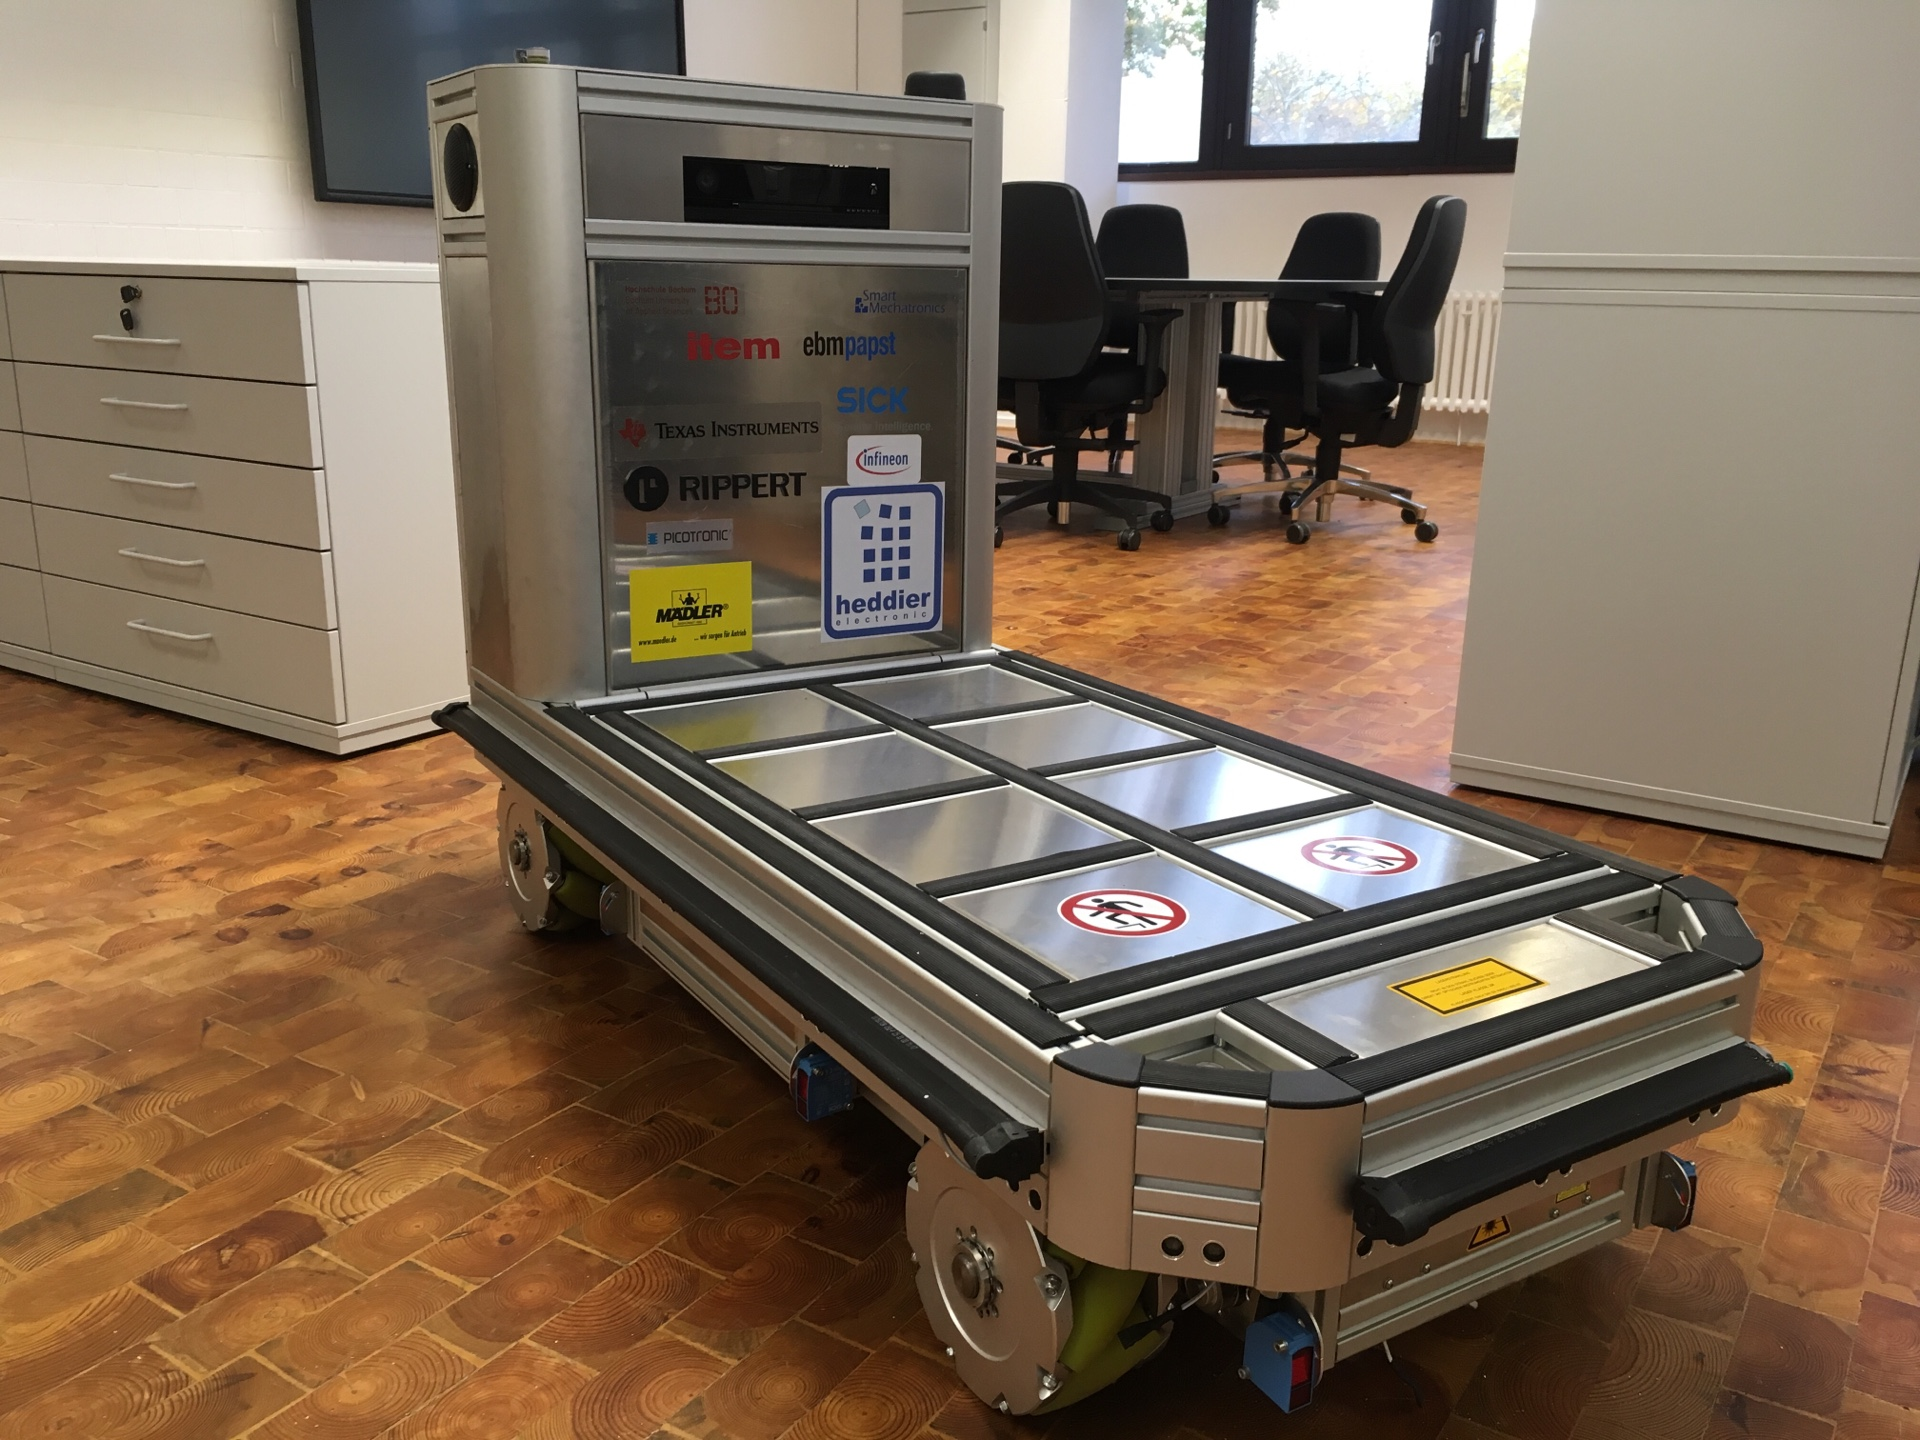
\includegraphics[angle=90,width=0.9\textwidth]{Bilder/Bild.jpeg}
						\caption{Abbildung des autonomen Logistikfahrzeugs ALF.}
						\label{fig: Wirkstruktur Schlupfregelung}
					\end{figure}
					
				
				
				
					\newpage 
					
				
					
					\section{Inhalt Datenträger} 
					\label{dataCD}
					\begin{enumerate}[label=\textbf{\arabic*},ref=A.1.\arabic*]
						\item Masterthesis in digitaler Form
						\label{it: dig}
						\item Entwickelte Software
						\label{it: Software}
						\item Lastenheft
						\label{it: Lastenheft}
						\item Literatur
						
					\end{enumerate}
				
		
	\end{appendix}
	
	
\end{document}